\documentclass[handout]{beamer} \usepackage[german]{babel}
\usepackage[utf8]{inputenc}
\usepackage{textcomp}
\usepackage{eurosym}
\usetheme{Berkeley}
\usepackage{wrapfig}
\usecolortheme{whale}
\usepackage{hyperref}

% Metadaten
%\institute[Warpzone e.V.]{Warpzone e.V.}
\institute[Warpzone e.V.]{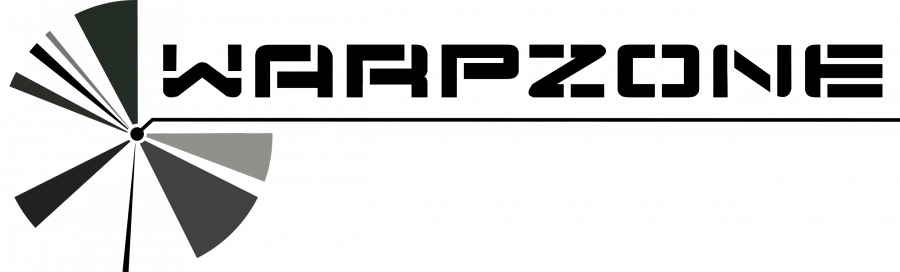
\includegraphics[height=20mm]{btcvortrag/wz.png}}
\author{blueling und Deaddy}
\date{2011-07-09}
 
\title[Bitcoin]{
Bitcoin - eine kryptographische P2P-Währung
}
%stylings
\setbeamertemplate{footline}[frame number]
\logo{
\includegraphics[height=10mm]{btcvortrag/BC_Logo_.png}}
%\titlegraphic{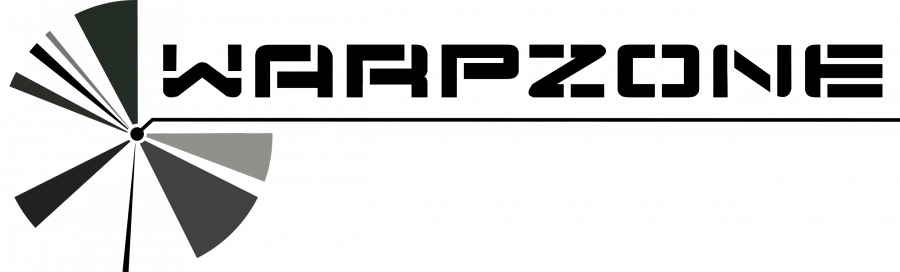
\includegraphics[height=20mm]{btcvortrag/wz.png}}

\AtBeginSection[]
{
   \begin{frame}
       \frametitle{Outline}
       \tableofcontents[currentsection]
   \end{frame}
}

\begin{document}
\begin{frame}
	\titlepage
\end{frame}

\section{Einführung}

\begin{frame}{Überblick über Bitcoin}
	\begin{itemize}
		\item erste {\bf dezentrale} digitale Währung
		\item 8 Seiten Paper 2008 unter Pseudonym 'Satoshi Nakamoto'
			veröffentlicht
		\item Wurzeln in der Cypherpunk-Bewegung (z.B. Wai Dai, b-money (1998))
		\item 2009 erste Implementation von Satoshi released
		\item community driven open source Projekt \\
			(http://bitcoin.org (Wiki,
			Forum), \#bitcoin
			auf freenode)
	\end{itemize}
\end{frame}

\begin{frame}
	{Problem?}
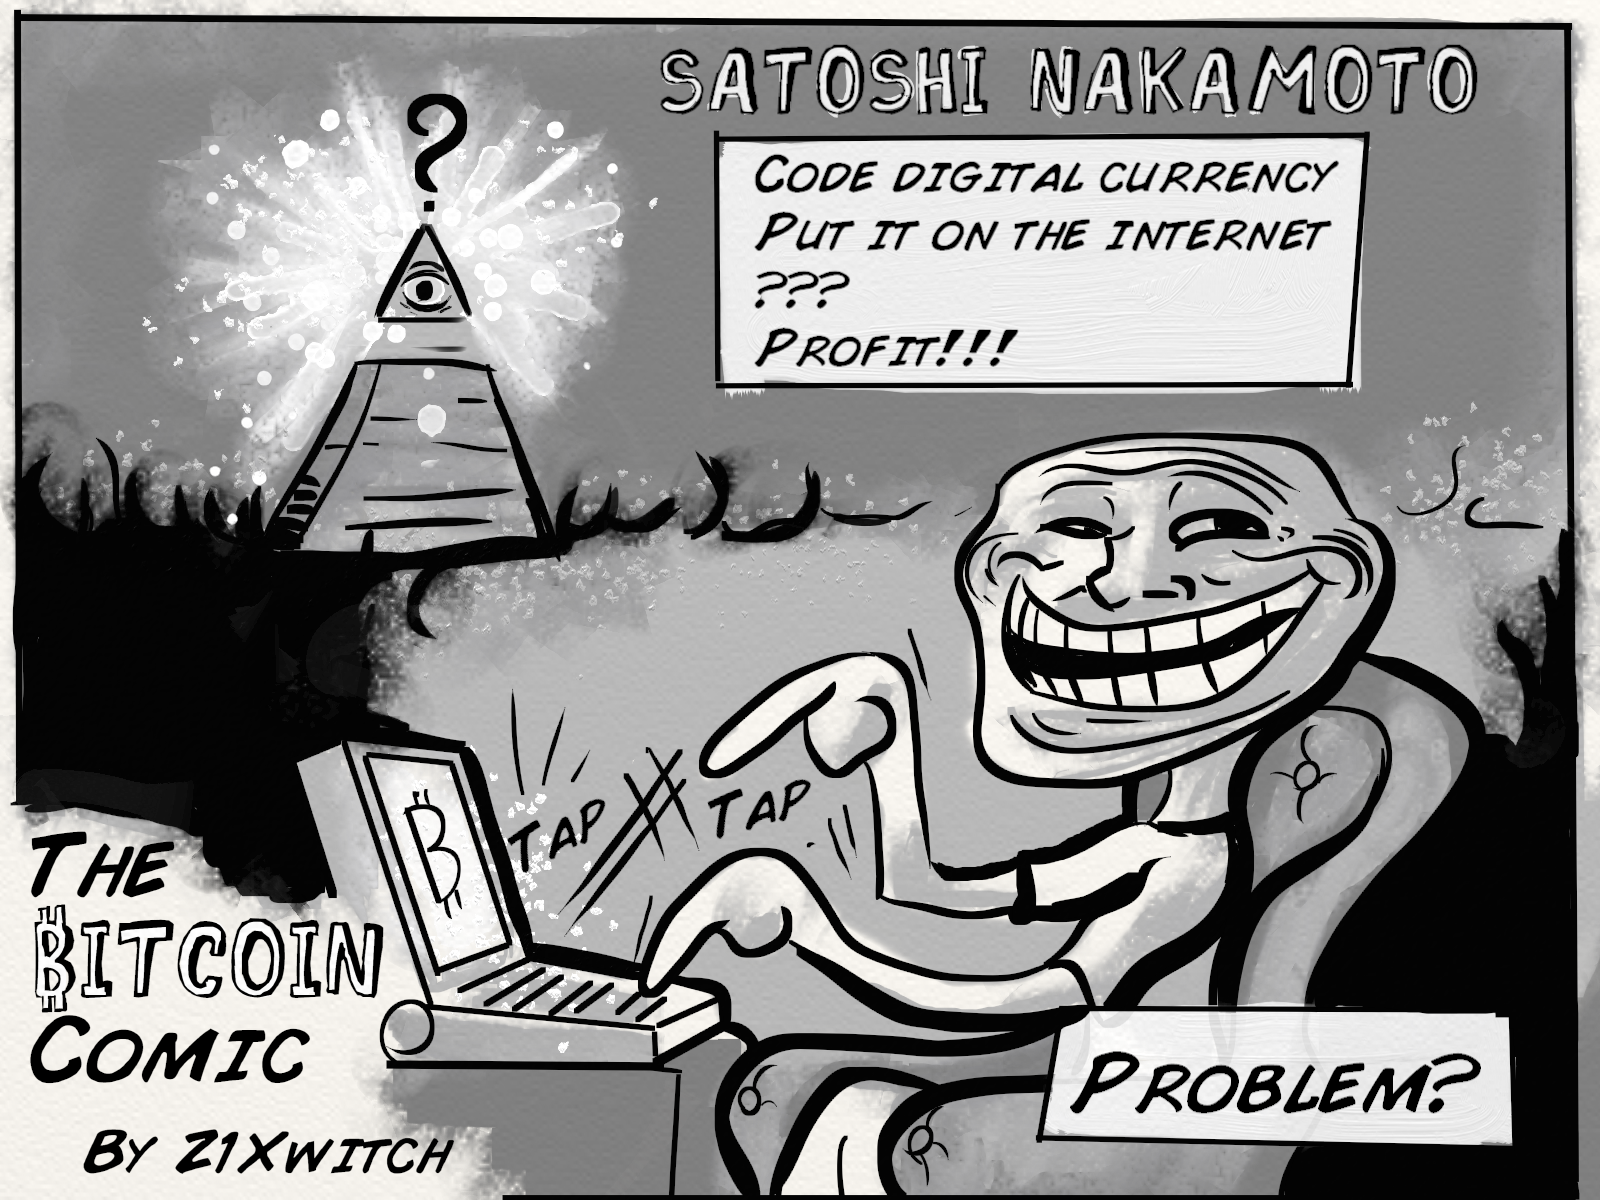
\includegraphics[height=60mm]{btcvortrag/satoshi-nakamoto-comic.png}
\end{frame}

\begin{frame}{Features}
	\begin{itemize}
		\item (bedingt) anonym
		\item grenzüberschreitend
		\item schnell
		\item dezentral
		\item kostengünstig
		\item fälschungssicher
		\item staatsunabhängig
		\item viral
	\end{itemize}
\end{frame}

\section{Bitcoins aus Usersicht}
\begin{frame}{Bitcoins aus Usersicht}
	\begin{itemize}
		\item bitcoin-client für Windows/Linux/Mac unter MIT-Lizenz (GUI und CLI)
		\item für Überweisungen benötigt man nur die Empfängeradresse
			(Zeichenkette wie 13rigybYMphatCxAhKksDeozbWE1s6sP6L)
		\item beliebig viele eigene Empfängeradressen für Anonymität
		\item jede Adresse beliebig lange verwendbar
	\end{itemize}
\end{frame}


\begin{frame} {Bitcoin Client unter Windows}
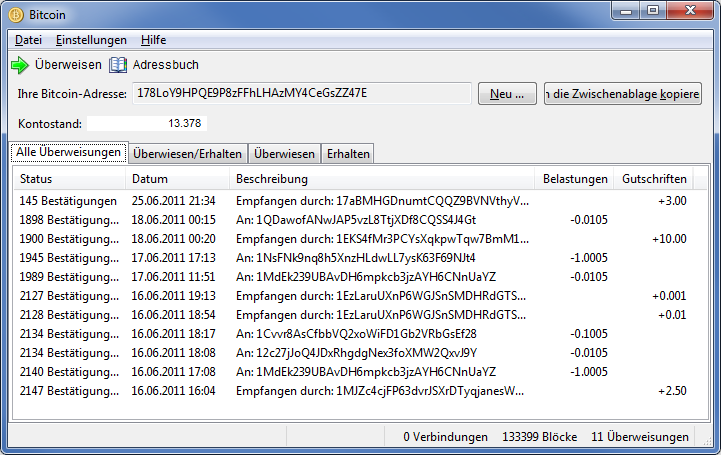
\includegraphics[height=60mm]{btcvortrag/BitcoinClientWindows.png}
\end{frame}

%\begin{frame}{Bitcoin Client aus Anwendersicht}
%	\begin{itemize}
%		\item gesamte Blockchain wird bei erstmaliger Nutzung heruntergeladen;
%		sonst fehlende Blöcke
%		%\item unter Windows im Autostart, nistet sich in TNA ein
%		\item Transaktion wird im Netz verteilt und deren Bestätigung im nächsten
%			Block erbeten
%	\end{itemize}
%\end{frame}

\begin{frame}{Durchführen einer Überweisung}
	\begin{itemize}
		\item Empfängeradresse, Betrag (+ evtl. Transaktionskosten)
			eingeben und absenden
		\item gültige Transaktion wird binnen ca. 10 Minuten das erste mal
			bestätigt; der Empfänger sieht die unbestätigte Transaktion gewöhnlich
			bereits nach wenigen Sekunden
		\item 6 Blöcke (etwa 1h) später wird die Transaktion als offiziell bestätigt
			angezeigt
		\item Bitcoins können erst nach Bestätigung ausgegeben werden
	\end{itemize}
\end{frame}

\begin{frame}{Einheiten}
	\begin{itemize}
		\item BTC als Währungsabkürzung in Anlehnung an ISO-4217
		\item \textbaht \ inoffizielles Währungssymbol (von der thailändischen Währung Baht)
		\item jeder Bitcoin auf bis 8 Nachkommastellen teilbar, kleinste Einheit
			1 Satoshi, also ein $\mu$\textbaht = 100 Satoshi
	\end{itemize}
\end{frame}

\section{Technik hinter Bitcoin}
\begin{frame}{Transaktionen}
	Transaktionen basieren auf asymmetrischer Verschlüsselung
	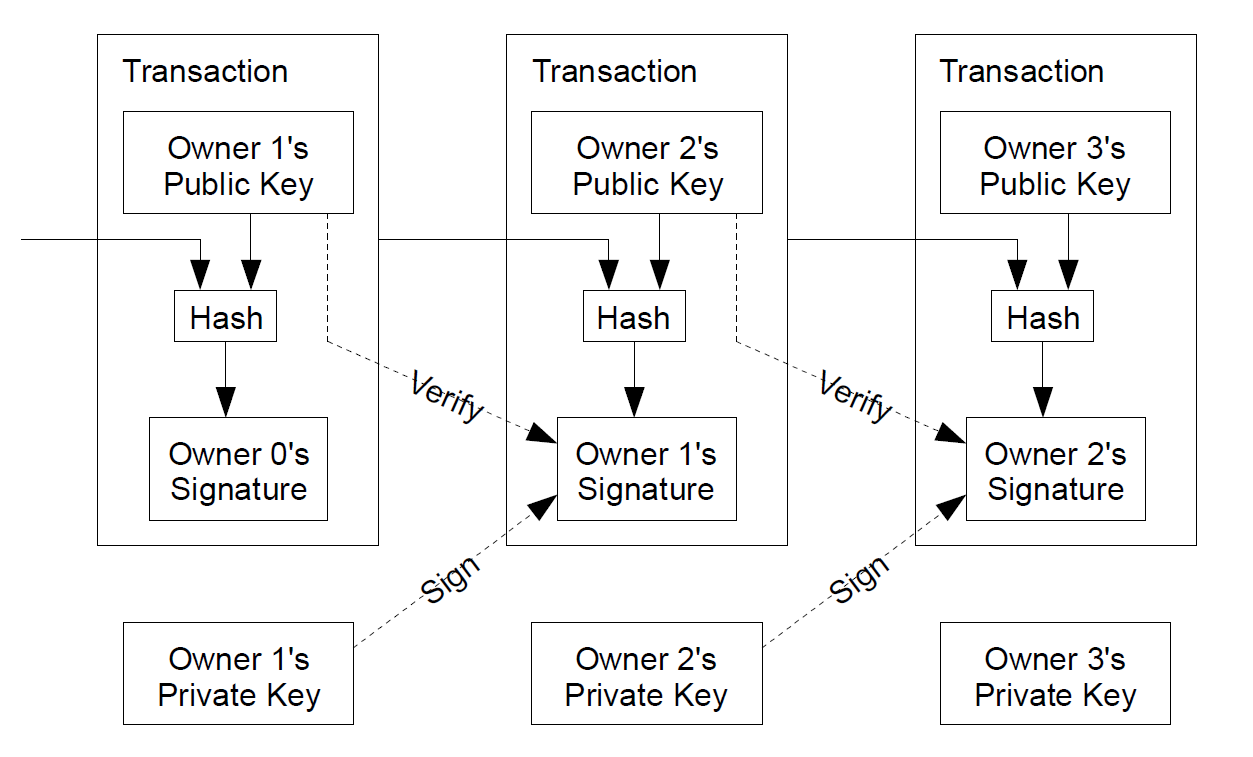
\includegraphics[height=60mm]{btcvortrag/TransactionChain.png}
\end{frame}

\begin{frame}{wallet.dat}
	\begin{itemize}
		\item Keyring für die eigenen Adressen und Transaktionen
		\item bei Verlust ist das Geld unwiderruflich verloren
		\item (noch) keine built-in Verschlüsselungs- oder Backupmechanismen
		\item Viren und Metasploitmodule sind im Umlauf
	\end{itemize}
\end{frame}


\begin{frame}{Probleme bei digitalen Transaktionen}
	\begin{itemize}
		\item "`double-spending"' verhindern erfordert Klärung der chronologischen Abfolge von Transaktionen
		\item vor Bitcoins setzte dies eine vertrauenswürdige Zentralinstanz
			voraus
	\end{itemize}
	Wie löst man das dezentral?
\end{frame}

\begin{frame}{Lösung: Distributed timestamp server}
	\begin{itemize}
		\item Transaktionen werden über Flooding-Algorithmus in das Netz
			gebroadcastet
		\item Transaktionen werden in Blöcken zusammengefasst und signiert,
			dabei enthält jeder Block den Hash des vorherigen Blocks
		\item es entsteht die sogenannte "`Blockchain"'
	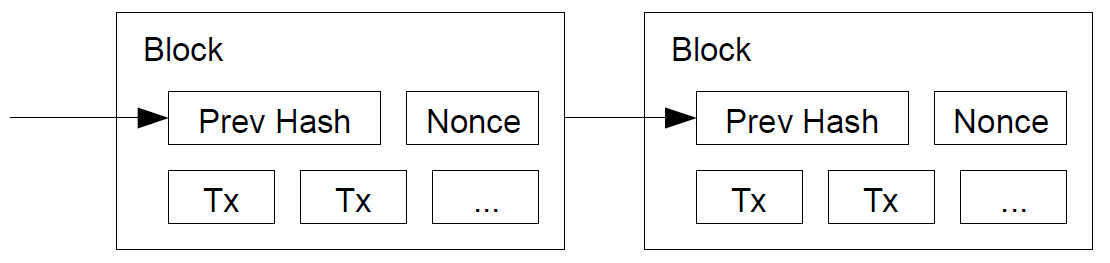
\includegraphics[height=20mm]{btcvortrag/ProofOfWorkChain.png}
	\end{itemize}
\end{frame}

\begin{frame}{Bestätigung eines Blocks}
	\begin{itemize}
		\item zur Bestätigung eines Blocks muss mit einer Nonce
			ein SHA-256-Hash gefunden werden, der kleiner als das aktuelle Target
			ist (anschaulich Anzahl der 0-bits am Anfang des Hashes)
		\item der Schwierigkeitsgrad wird protokollseitig über einen gleitenden
			Durchschnitt alle 2016 Blöcke (ca. 2 Wochen) so angepasst, dass im Schnitt alle 10 Minuten ein Block
			berechnet wird
	\end{itemize}
\end{frame}

\begin{frame}{Blockchain}
	\begin{tabular}{l l}
	\begin{minipage}{0.7\textwidth}
	\begin{itemize}
		\item längste Kette ist offiziell und wird als Grundlage für den nächsten
			Block genommen
		\item	"`Länge"' ist die Gesamtschwierigkeit für die Blockchain
		\item gibt es zwei gleichlange Ketten, rechnet die Node nur an der zuerst
			erhaltenen und verwirft diese, falls die andere früher erweitert wird
	\end{itemize}
	\end{minipage}
	&
	\begin{minipage}{0.3\textwidth}
	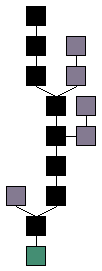
\includegraphics[width=20mm]{btcvortrag/Blockchain.png} 
	\end{minipage}
\end{tabular}

\end{frame}

\begin{frame}{Wer berechnet die Blockchain?}
	\begin{itemize}
		\item jeder kann sich an der Hashberechnung beteiligen
		\item um die Blockchain durch eine manipulierte zu ersetzen (z.B. für
			double-spending) muss man die Kette ab dem zu ändernden Block neu
			Berechnen (mit einer Difficulty $\geq $ der originalen Chain)
		\item mit $>50\%$ der Rechenleistung bestimmt man das Netzwerk
	\end{itemize}
\end{frame}

\begin{frame}{Sicherheit der Blockchain}
	Angriff auf die Blockchain ist ein binomialer Random-Walk und analog zum Gambler's Ruin problem: ein
	Spieler mit unendlichem Kredit startet mit einem Defizit und spielt eine
	möglicherweise unendliche Anzahl Spiele um dieses auszugleichen.
	Die Wahrscheinlichkeit $q_z$, dass er mit $z$ Blöcken Rückstand wieder aufholt ist
	\begin{equation*}
		q_z = \left\{\begin{array}{cl} 1, & \mbox{falls }p\leq q\\
			\left( q/p \right)^z, & \mbox{sonst} \end{array}\right.
	\end{equation*}
	wobei
		$p=$ Wahrscheinlichkeit, dass eine ehrliche Node den nächsten Block
			findet und
		$q=$ Wahrscheinlichkeit, dass der Angreifer den nächsten Block
			findet\\
	Besitzt der Angreifer $\geq 50\%$ der Rechenleistung, entspricht dies dem
	Fall $q\ge p$
\end{frame}


\section{Mining}
\begin{frame}{Mining}
	\begin{itemize}
		\item Blockchain-Berechnung ist rechenintensiv
		\item es gibt als Belohnung für die Erstellung eines Blocks anfangs 50BTC
			(halbiert sich alle 210k Blöcke/4 Jahre)
		\item zusätzlich erhält der Blockersteller etwaige (freiwillig zahlbare) Transaktionsgebühren
		\item der Miner bestimmt welche Transaktionen er aufnimmt (z.B. nur
			welche mit Transaktionsgebühren)
	\end{itemize}
\end{frame}

\begin{frame}{Mining}
	\begin{itemize}
		\item die Belohnung für das Finden von Block-Hashes ist die einzige Geldschöpfung
		\item hierdurch wird das Gesamtvolumen auf etwa 21 Millionen BTC (etwa
			2031 erreicht) begrenzt, bei der derzeitigen Aufteilung gibt es
			maximal $2,1\cdot10^{15}$ diskrete Einheiten
		\item derzeit befinden sich etwa 6.765.550 BTC im Umlauf (Stand: 08. Juli
			16 Uhr)
	\end{itemize}
\end{frame}

\begin{frame}
	{Entwicklung der Bitcoinmenge}
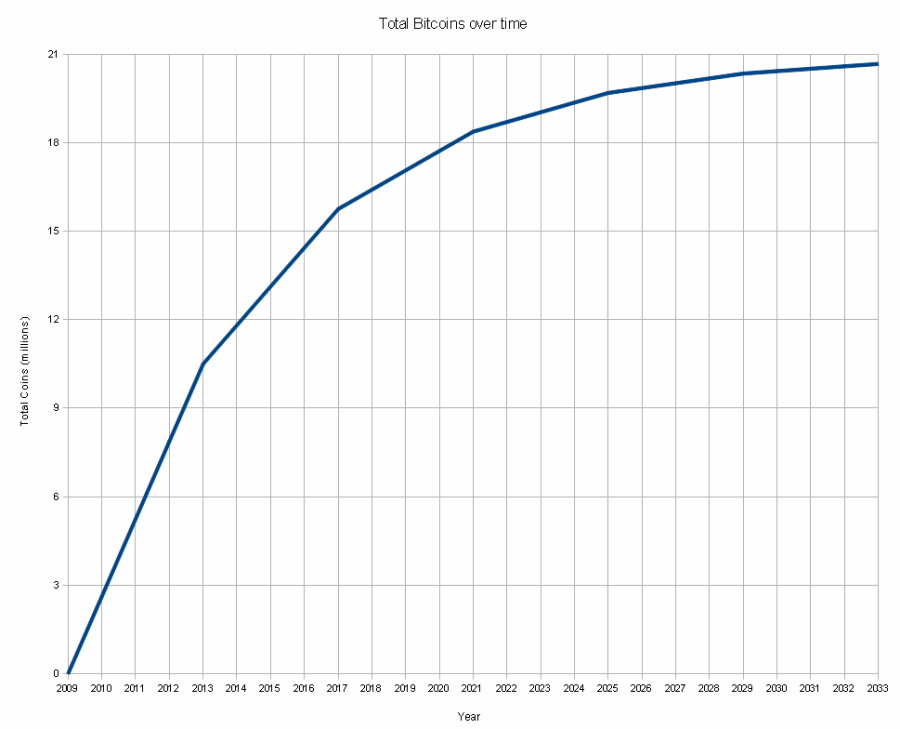
\includegraphics[height=70mm]{btcvortrag/Total_bitcoins_over_time.png}
\end{frame}

\begin{frame}{Rechenaufwand beim Minen}
	\begin{itemize}
		\item mit steigender Rechenleistung des Gesamtnetzes erhöht sich
			langfristig nicht die Anzahl der
			generierten Coins ($6\cdot50BTC/h$)
		\item Grenzkosten für die Profitabilität liegen bei den Energiekosten
			(bei aktuellem Kurs von etwa \$15 pro BTC bleibt Mining bis \$108k
			Energiekosten für das gesamte Netz profitabel)
		\item derzeit verwenden Miner hauptsächlich GPUs
		\item wegen Energieffizienz demnächst vermutlich hauptsächlich über
			dedizierte ASICs oder FPGAs
	\end{itemize}
\end{frame}

\begin{frame}{Typisches Mining-Rig}
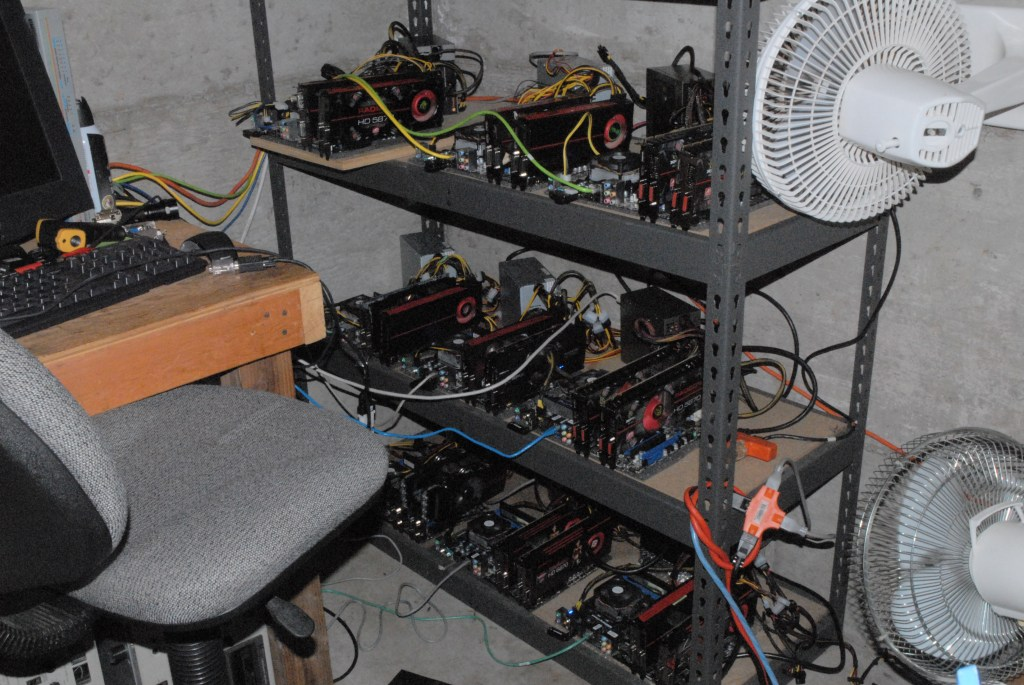
\includegraphics[height=70mm]{btcvortrag/mining-shelf.jpg}
\end{frame}

\begin{frame}{Weniger wirtschaftliches Mining-Rig}
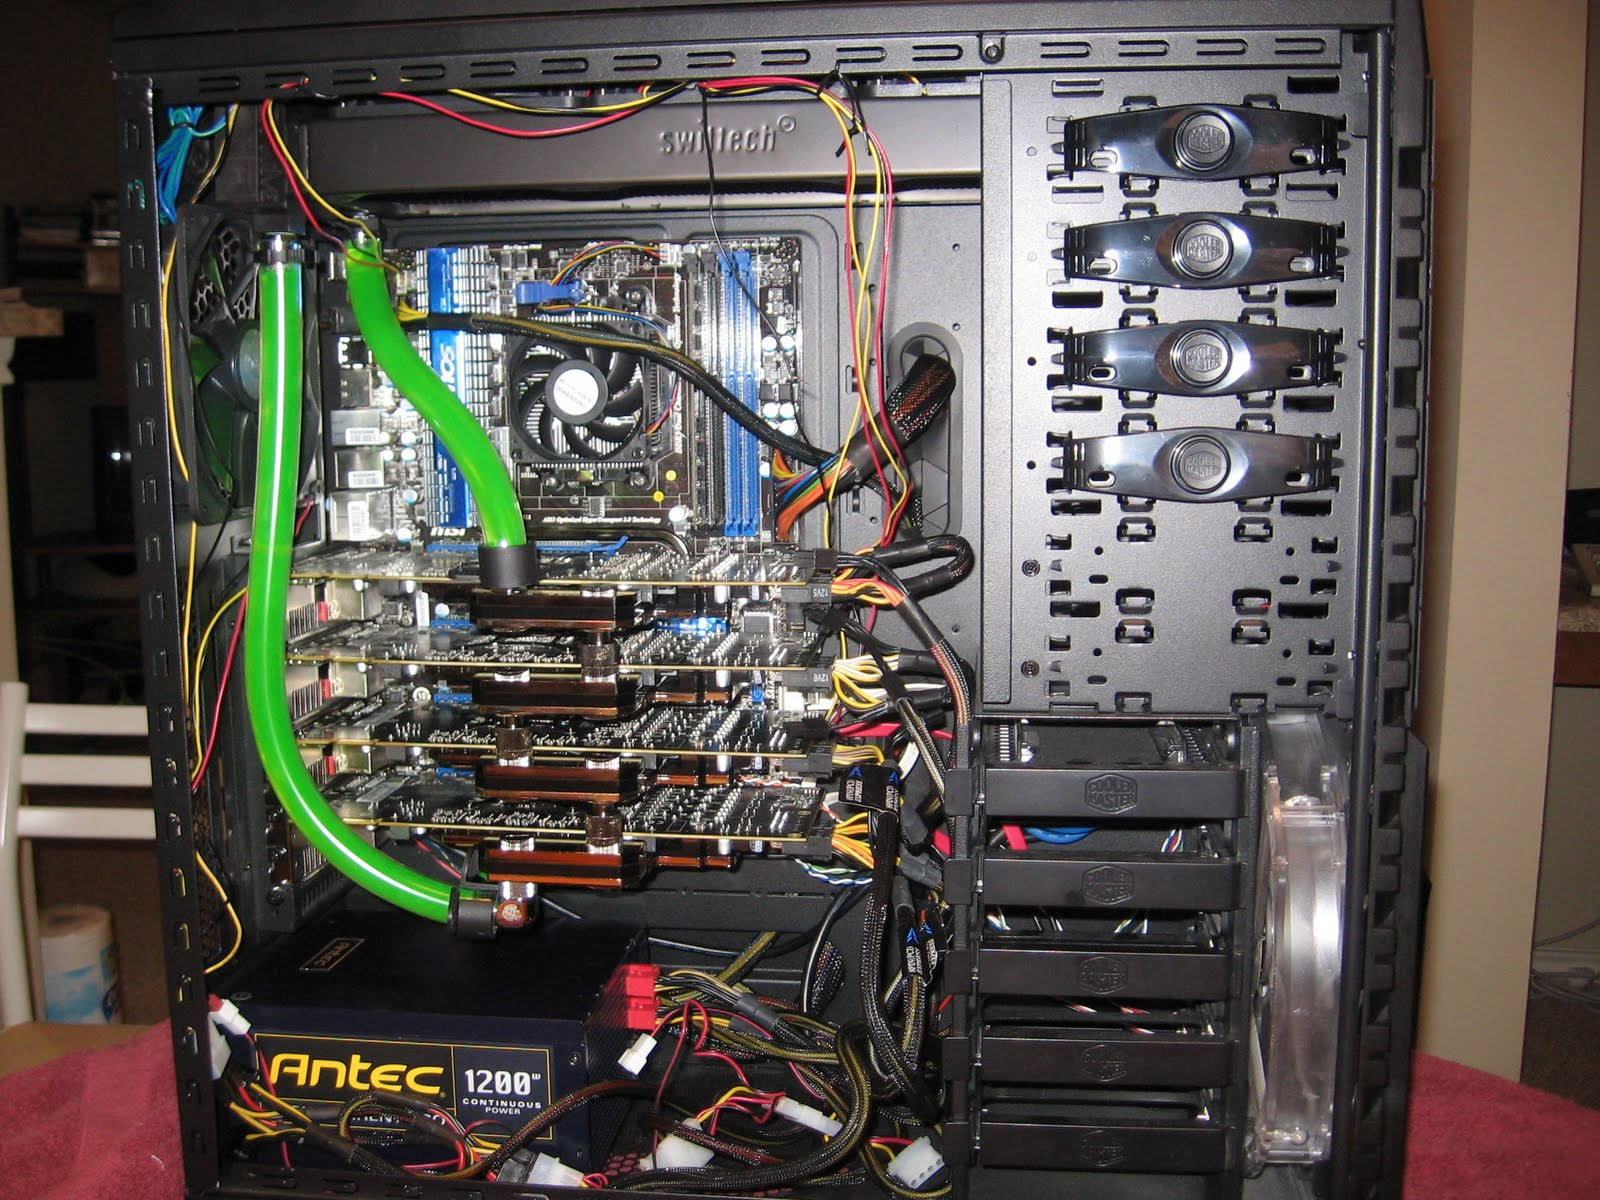
\includegraphics[height=70mm]{btcvortrag/liquid-cool-mining-rig.JPG}
\end{frame}

\begin{frame}{Preis-Leistungs-Sieger (Rackmount)}
	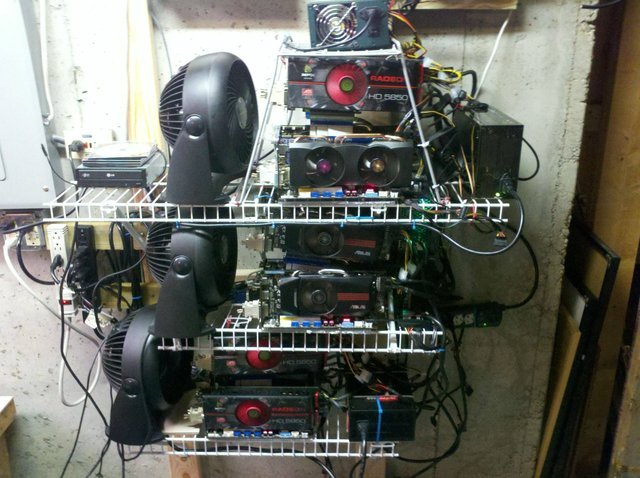
\includegraphics[height=70mm]{btcvortrag/rack-mounted-mining.jpg}
\end{frame}

%\begin{frame}{Mining-Pools}
%	\begin{itemize}
%		\item je mehr Teilnehmer, desto schwieriger wird es für den einzelnen
%			einen Block zu finden \\
%			$\Rightarrow$ Zusammenschluss in Mining-Pools
%		\item der Pool gibt Arbeitsblöcke mit niedrigerer Schwierigkeitgrad
%			heraus als das Netzwerk, diese lassen sich von Clients schneller
%			berechnen und dienen als Beleg der eingebrachten Arbeit
%		\item da SHA-256 Pseudozufallszahlen generiert, besteht nach wie vor die
%			gleiche Chance einen Block mit der Schwierigkeitsgrad des Netzes zu
%			finden
%	\end{itemize}
%\end{frame}

\begin{frame}{Kooperatives Minen im Pool}
	\begin{itemize}
		\item je größer das Netzwerk, desto schwieriger wird es für den einzelnen
			einen Block zu finden \\
			$\Rightarrow$ Zusammenschluss in Mining-Pools
		\item findet ein Teilnehmer einen Block, werden alle Poolteilnehmer
			proportional zur eingebrachten Rechenleistung entlohnt; es fällt ggf.
			eine Poolgebühr im einstelligen Prozentbereich an
		\item unabhängig von Pool- oder Solomining ist der durchschnittliche 
			$Ertrag/h \approx \frac{eigene Hashleistung}{gesamte Hashleistung des
			Netzes}\cdot6\cdot50 BTC/h$
		\item mit steigender Poolgröße wird die Varianz des Ertrags reduziert,
			auf lange Sicht wird der Gesamtertrag aber kaum geändert (nur
			Poolgebühren und evtl. Grenzeffekte wenn die generierten Coins gegen 0
			gehen)
	\end{itemize}
\end{frame}

\begin{frame}{Hashrate-Verteilung}
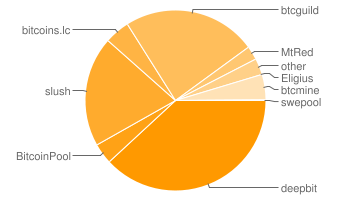
\includegraphics[height=45mm]{btcvortrag/hashratedistribution.png}
\end{frame}

\begin{frame}{Kann man mit Mining reich werden?}
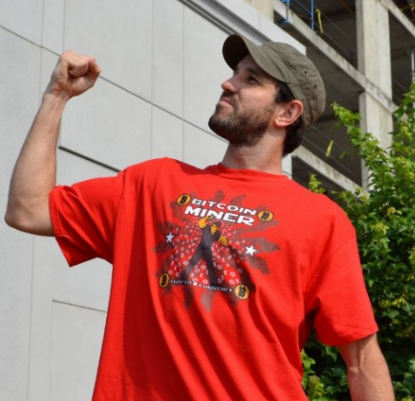
\includegraphics[height=70mm]{btcvortrag/MiningTshirt3.jpg}
\end{frame}

\begin{frame}{Kann man mit Mining reich werden?}
	\begin{itemize}
		\item Early Adopters haben definitiv profitiert; risikoreich für
			Neueinsteiger
		\item Energiekosten drücken den Gewinn
		\item Beispiel-Miner mit 2 HD 5850 hat etwa tägliche Stromkosten von 1,50 EUR, generiert derzeit
			0.35 BTC pro Tag, das entspricht etwa 3,50 EUR, es
			bleiben also nur 2€ Gewinn pro Tag (Stand 08. Juli)
		\item aktueller Mining-Tagesertrag lässt sich nicht extrapolieren: Preis
			treibt Difficulty
	\end{itemize}
\end{frame}

\begin{frame}{Entwicklung der Mining-Leistung}
	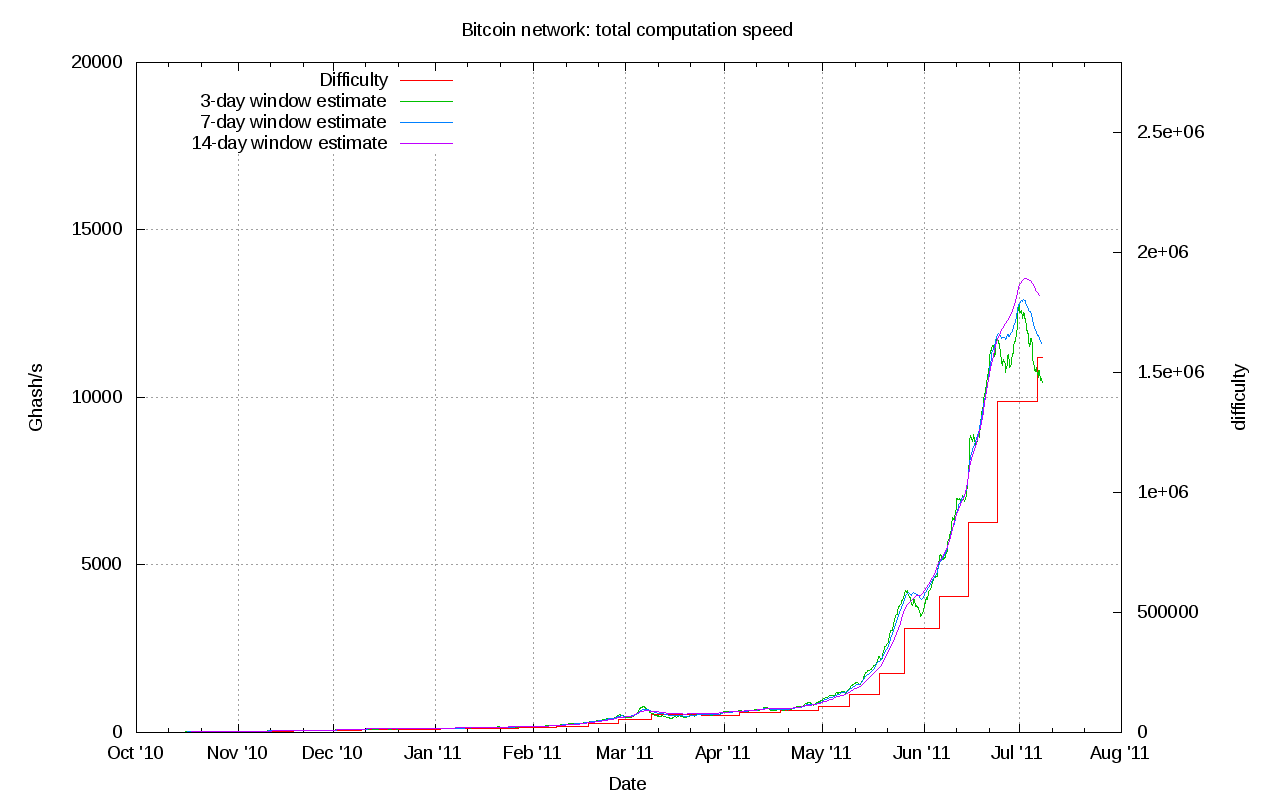
\includegraphics[height=60mm]{btcvortrag/speed-lin.png}
\end{frame}

\begin{frame}{Kann man mit Mining reich werden?}
	\begin{itemize}
		\item dedizierte FPGA/ASIC-Miner-Boards in Aussicht
		\item GPU vs. CPU Energieeffizienz liegt bei 10:1 \\
			ASIC vs. GPU vermutlich auch
		\item wer auf steigende Preise hofft, kann BTCs besser kaufen als sie
			selbst zu minen
		\item Mining aus Spaß an der Freude (vgl. Folding@Home, SETI@home)
			ist natürlich immer möglich
	\end{itemize}
\end{frame}

\begin{frame}{Erste Aussteiger}
	\begin{itemize}
		\item Mining-Rig-Verkäufe nehmen zu
	\end{itemize}
	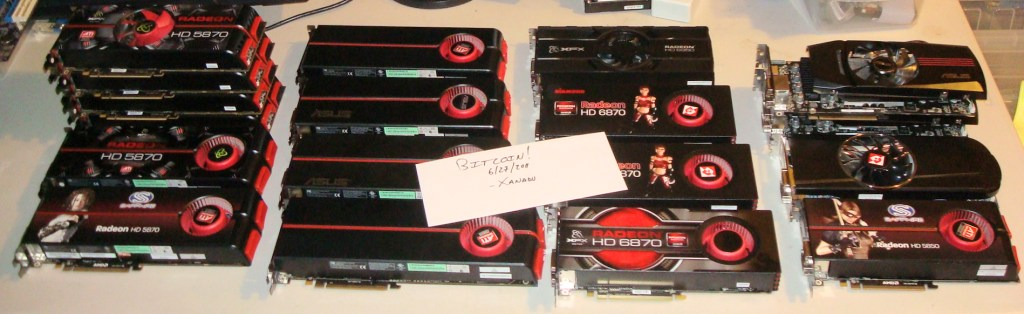
\includegraphics[height=30mm]{btcvortrag/aussteiger.jpg}
\end{frame}

\section{Ökonomie}
\begin{frame}{Währungsentwicklung - eine Blase?}
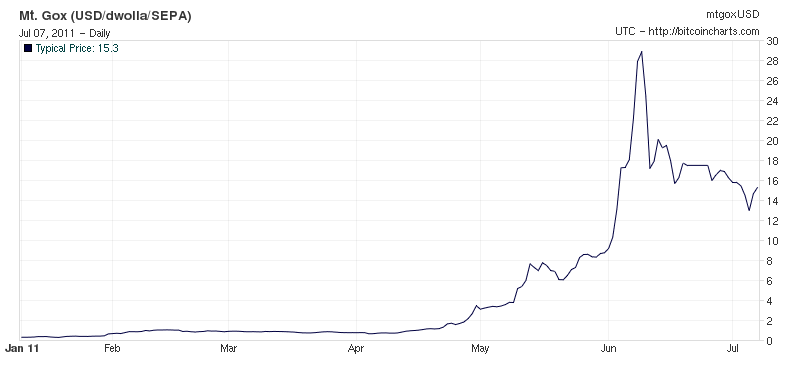
\includegraphics[height=45mm]{btcvortrag/bitcoin-price-mtgox-simple.png}
\end{frame}

\begin{frame}{Währungsentwicklung in Zahlen}
	\begin{tabular}[ht]{l|c}
		\hline
		Zeitraum & Preis in USD \\
		\hline\hline
		2010/10						&	~0,06 \\
		2010/11--2011/01			&	0,2--0,5 \\
		2011/01--2011/04			&	0,5--1 \\
		2011/04--2011/06			&	1--30 \\
		8. Juni						&	31.5 (All-Time-High)\\
		10.--11. Juni				&	Crash von 30 auf 15\\
		2011/07						&	15\\
		\hline
	\end{tabular}
\end{frame}


\begin{frame}
	{Grundlagen der Ökonomie}
	\begin{itemize}
		\item BTC sind ein limitiertes Gut, welches nicht nach Belieben erzeugt
			werden kann\\
		\item BTC lassen sich {\bf echt übertragen}, sie werden nicht einfach nur
			kopiert\\
			$\Rightarrow$ 
			sie eignen sich als digitales Tauschmittel
		\item BTC eignen sich für grenzüberschreitende Bezahlvorgänge
		\item Teilnahme am System für jedermann möglich
	\end{itemize}
\end{frame}

\begin{frame}{Startschwierigkeiten}
	\begin{itemize}
		\item Währungsfunktion hängt von anhaltender Bereitschaft "`offizielles"'
			Geld in BTC zu tauschen ab
		\item Kreislauf: Kunde tauscht lokale Währung in BTC, bezahlt
			Gut/Dienstleistung in BTC, Händler/Anbieter tauscht BTC in lokale
			Währung und deckt seine Kosten
		\item es existieren kaum Angebote mit fixen BTC-Preisen, Bezugsgröße sind
			Preise in USD, EUR etc.
	\end{itemize}
\end{frame}

\begin{frame}{Essen für BTC}
	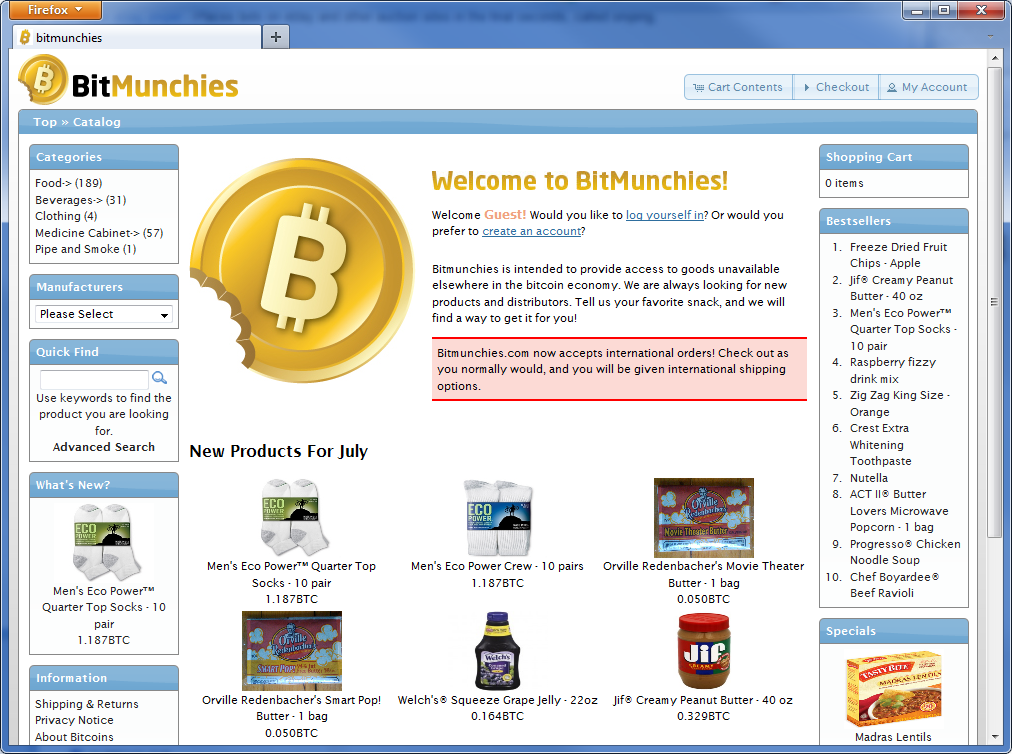
\includegraphics[height=60mm]{btcvortrag/Bitmunchies.png}
\end{frame}

\begin{frame}{Hardware für BTC}
	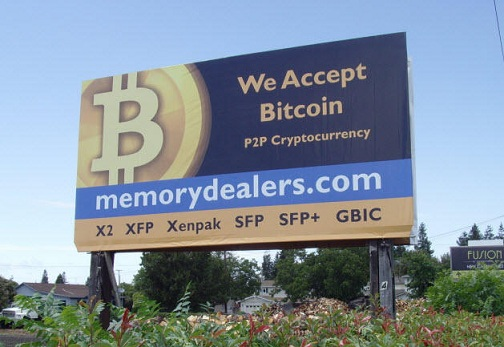
\includegraphics[height=60mm]{btcvortrag/bitcoin-billboard.jpg}
\end{frame}

\begin{frame}{Exchanges}
	\begin{itemize}
		\item Online-Händelsplätze mit Verrechnungskonto bei denen
			ähnlich wie bei Wertpapier-Online-Brokern gehandelt wird,\\
			z.B. Mt.  Gox, tradeHill, bitcoin7
		\item Escrow-Handelsplattformen bei denen ein Orderbook, aber kein
			Währungskonto geführt wird, BTC-Betrag
			wird treuhänderisch verwaltet
		(Geldtransfer läuft außerhalb bspw. über Überweisungen),\\
		 z.B. bitmarket.eu 
	\end{itemize}
\end{frame}

\begin{frame}{Handel außerhalb von Exchanges}
	\begin{itemize}
		\item neben Überweisungen sind anonyme Barzahlungen oder
			Bargeld-Versand per Brief gängig
		\item OTC Handel per IRC-Channel \#bitcoin-otc-foyer auf freenode.net
		\item Vereinzelt existieren BTC-Meetups/User groups/Stammtische
		\item Hacker/Geeks Deines Vertrauens
	\end{itemize}
\end{frame}

\begin{frame}{Beispiel: Mt. Gox}
	\begin{itemize}
		\item Mt. Gox wird von Tibanne Co. Ltd. (Japan) betrieben, EUR
			SEPA Überweisungen laufen aber von/zu einem Konto in Frankreich und
			werden zum EZB-Kurs in USD getauscht
		\item teils wird eine API (RESTful) für eigene automatische
			Handelssysteme angeboten
		\item Angebot soll für Trader ausgeweitet werden: Margin- und
			Optionshandel, Leerverkäufe etc.; derzeit hauptsächlich nur primitive
			Limit-Orders möglich
		\item keine Verträge oder Sicherheiten
	\end{itemize}
\end{frame}

\begin{frame}{Mt. Gox Webseite}
	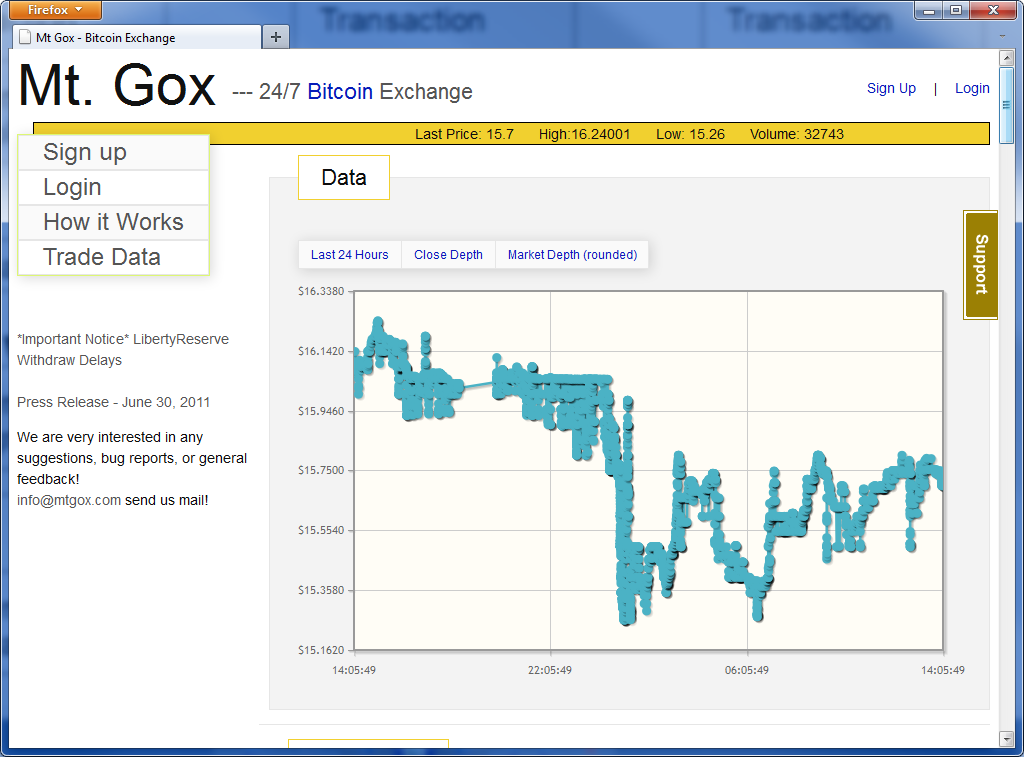
\includegraphics[height=70mm]{btcvortrag/MtGox.png}
\end{frame}

\begin{frame}{Deflation}
	\begin{tabular}{l l}
	\begin{minipage}{0.6\textwidth}
	\begin{itemize}
		\item Bitcoins sind ein Gegensatz zu gängigen Fiat-Währungen, die vom
			Staat per Beschluss erzeugt und gewollt inflationiert werden
		\item inflationäre Fiat-Währungen (unser Weltwährungssystem) sind wegen
			des exponentiellen Wachstums nicht aufrechtzuerhalten
	\end{itemize}
	\end{minipage}
	&
	\begin{minipage}{0.4\textwidth}
	
\includegraphics[width=35mm]{btcvortrag/helicopter-ben.jpg}
\end{minipage}
	\end{tabular}
\end{frame}

\begin{frame}{USD-Geldmenge}
	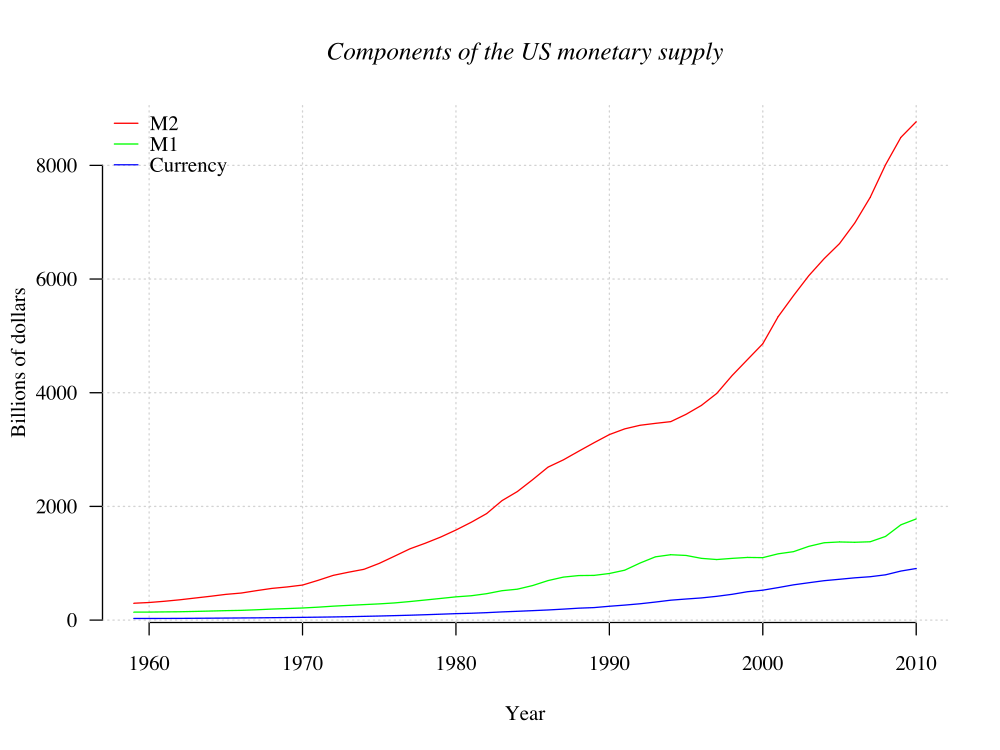
\includegraphics[height=75mm]{btcvortrag/usd-geldmenge.jpg}
\end{frame}

\begin{frame}{Wirtschaftliche Kritik an BTC}
	\begin{itemize}
		\item BTC-Geldmenge kann nicht durch zentrale Instanz angepasst werden
			(vgl. rohstoffgedeckte Währung)
		\item Deflationsspirale befürchtet: bei steigender Kaufkraft der Währung leiden Schuldner
		\item Folgen: Horten von BTC als Wertaufbewahrungs- oder
			Spekulationsobjekt, Kaufzurückhaltung
		\item Kreditvergabe und Fractional Banking auch mit BTC möglich
	\end{itemize}
\end{frame}

%
%\begin{frame}{Bitcoins als Währung}
%	\begin{itemize}
%		\item schlechteres Geld verdrängt besseres Geld als Zahlungsmittel
%		\item Folge: eingeschränkte Währungsfunktion, da man lieber in
%			"`schlechten"' USD oder EUR bezahlt
%	\end{itemize}
%\end{frame}

\begin{frame}
	{Rechtslage}
	\begin{itemize}
		\item kein staatlich anerkanntes oder verbindliches Zahlungsmittel
		\item noch keine Präzedenzfälle bekannt
		\item Stress mit dem Finanzamt vorprogrammiert
		\item steuerlich vermutlich keine Währung, sondern Ware\\
			$\Rightarrow$ MwSt. muss abgeführt werden
	\end{itemize}
\end{frame}

\begin{frame}
	{Legalität}
	\begin{itemize}
		\item im privaten Bereich ist der gelegentliche Handel vmtl. bis \EUR{600}/Jahr
			steuerfrei (§23 EStG)
		\item fraglich: ist der Handel mit BTC aktive Teilnahme an organisierter
			Geldwäsche?
		\item Interessenlage des Staates bzgl. BTC dürfte klar sein
	\end{itemize}
\end{frame}

\section{Zwischenfälle und Angriffszenarien}



%\begin{frame}
%	{LSHIFT- und RETURN-Bugs (28. Juli 2010)}
%	\begin{itemize}
%		\item ersterer führte auf einigen Maschinen zum Absturz
%		\item zweiterer erlaubte es Coins auszugeben, die einem nicht gehörten
%		\item wurde auf dem Testnetwork demonstriert und in Bitcoin 0.3.5 gefixt
%	\end{itemize}
%\end{frame}
%
%\begin{frame} {OP\_CHECKSIG (29. Juli 2010)}
%	\begin{itemize}
%		\item Transaktionen konnten unbegrenzt viele OP\_CHECKSIG-Befehle enthalten
%		\item ermöglichte DDoS-Angriff
%		\item gefixte Bitcoin-Version wurde umgehend released
%	\end{itemize}
%\end{frame}

\begin{frame}
	{Overflow Bug (15. August 2010)}
	\begin{itemize}
		\item Block 74638 enthielt eine TX, die für zwei Adressen insgesamt 184
			Milliarden BTC erzeugte
		\item Blockchain musste geforked werden
		\item trotz einiger ungepatchter Nodes überholte die neue Chain
			schließlich die mit der Fehlbuchung
	\end{itemize}
\end{frame}

\begin{frame}
	{Mt. Gox-Hack (25. Juni 2011)}
	\begin{itemize}
		\item BTC-Kurs fiel innerhalb weniger Minuten von USD 17,5 auf USD 0,01
		\item offizielle Ursache: Konto mit administrativem Zugriff (von jemandem
			der als externer Audits durchführt) wurde kompromittiert und
			ermöglichte die Ausschüttung sehr vieler, nur in der Datenbank von Mt.
			Gox existierender Bitcoins
		\item kurz darauf war eine .csv-Datei mit allen Mt. Gox-Accounts für
			jeden herunterladbar
	\end{itemize}
\end{frame}

\begin{frame}
	{Folgen des MT. Gox-Hacks}
	\begin{itemize}
		\item Handel wurde eine Woche eingestellt, es wurde ein Rollback der
			Transaktionen durchgeführt, Mt. Gox ersetzte die ~1000 BTC die vom
			Angreifer ausgezahlt werden konnten aus eigener Tasche
		\item Handel startete erstaunlich ruhig wieder; Trading-API erst einige
			Tage später wieder voll funktionstüchtig
		\item "`goxed"' bürgerte sich als Meme in der Bitcoin-Community ein
	\end{itemize}
\end{frame}

\begin{frame}{Kurs/Volumen während des Hacks}
	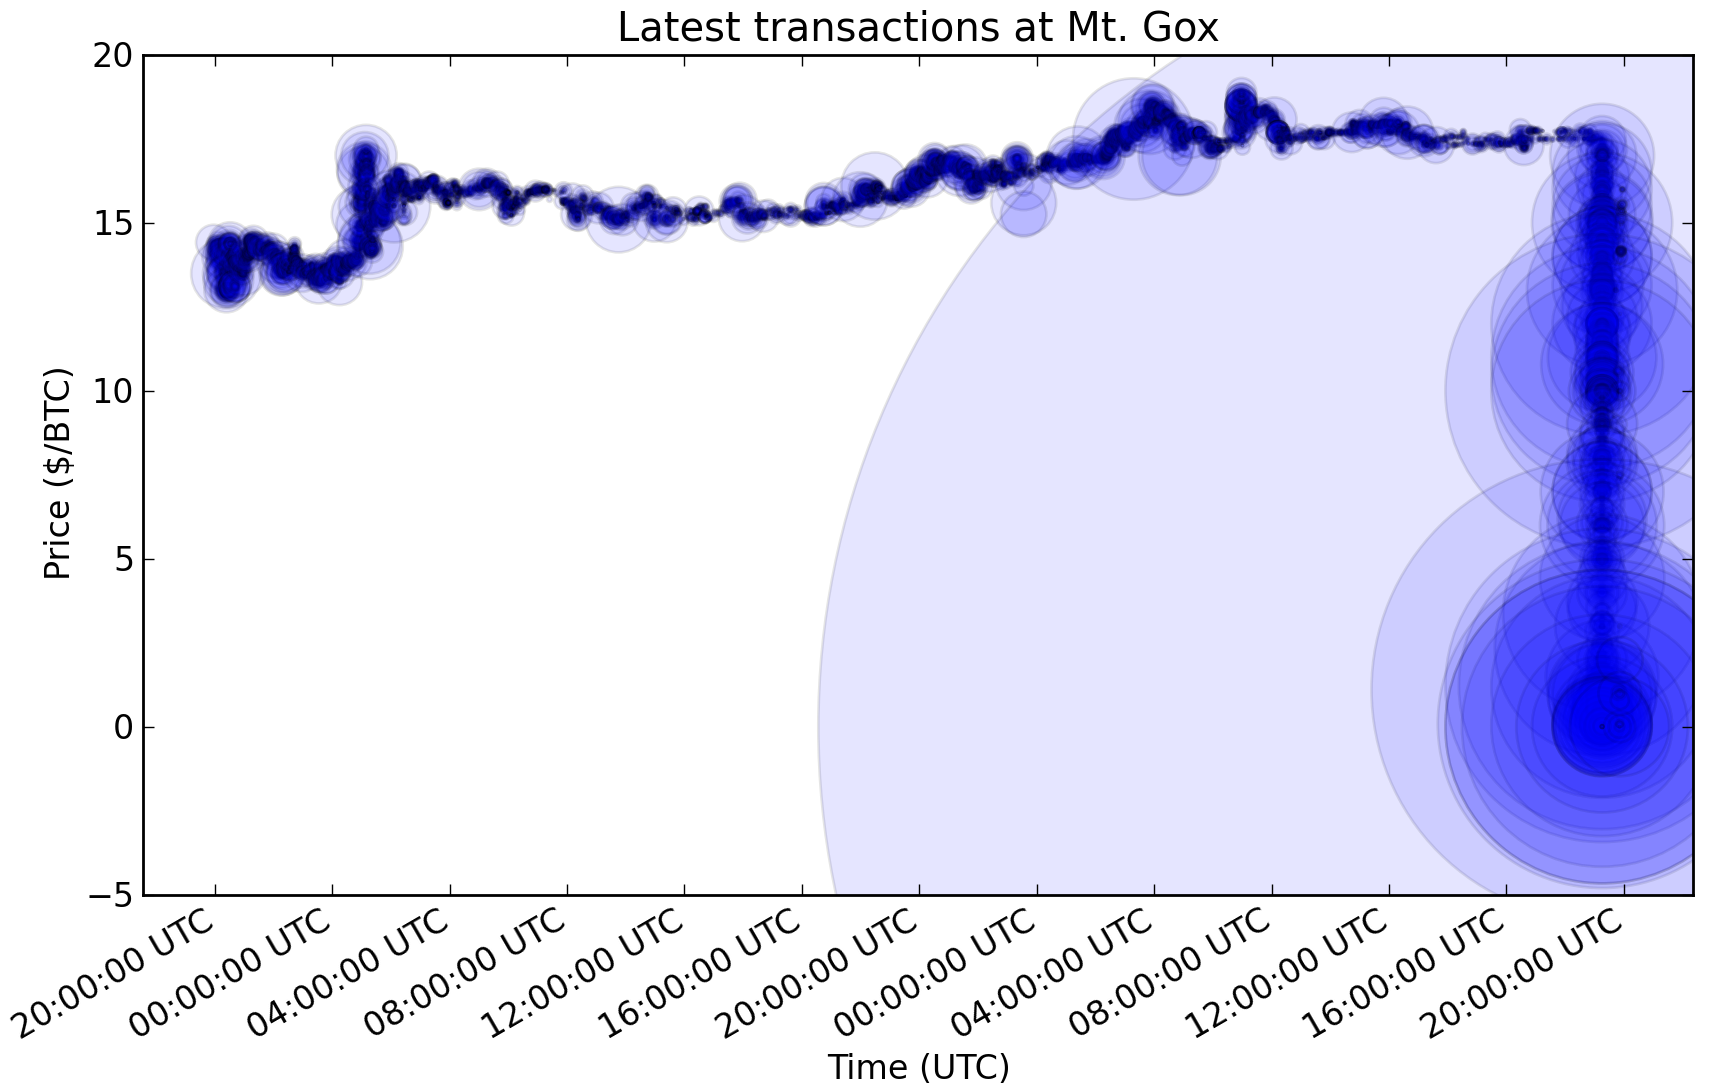
\includegraphics[height=60mm]{btcvortrag/mtgox-crash.png}
\end{frame}

\begin{frame}{Huch}
	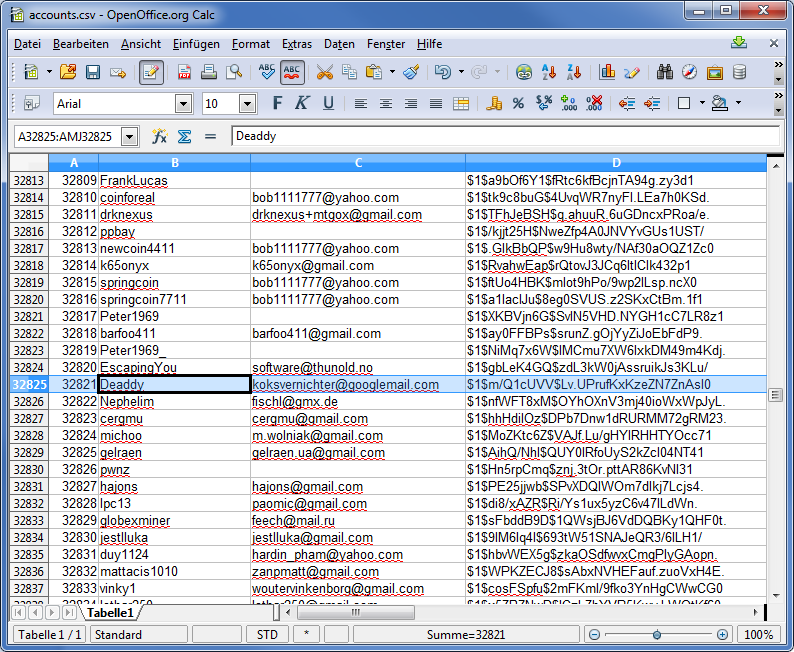
\includegraphics[height=60mm]{btcvortrag/MtGoxLeakDeaddy.png}
\end{frame}

\begin{frame}
	{Weitere Angriffszenarien}
	\begin{itemize}
		\item Timejacking: durch das Einhashen einer falschen Netzwerkzeit (eine
			Node verwirft Blöcke erst ab 2h Diskrepanz zur eigenen Zeit) kann man
			ggf. einzelne Nodes mit einer falschen Blockchain isolieren und falls
			man es schafft, dem Client 6 falsche Blöcke zu senden, würden
			Transaktionen als bestätigt erscheinen
		\item Cancer Nodes: mit sehr vielen IPs die sich in den höchsten 16 Bits
			unterscheiden kann man im IRC-Bootstrap-Channel ein Netzwerk aus bösen
			Clients aufbauen, mit welchem man zumindest störende Aktionen fahren
			kann
	\end{itemize}
\end{frame}


\begin{frame}
	{Quellen und Links}
	\begin{itemize}
		\item \url{http://www.bitcoin.org/} -- Hauptseite des Projekts: Infos, Wiki, Forum                                      
		\item \url{http://blockexplorer.com/} -- Überweisungen tracken etc.                                                    
		\item \url{http://www.weusecoins.com/} -- Erklärung von Bitcoin für Non-Geeks                                          
		\item \url{http://bitcoin.sipa.be/} -- Bitcoin Network Charts                                                          
		\item \url{http://bitcoincharts.com/} -- Marktübersicht 
	\end{itemize}
\end{frame} 
\end{document}
